\documentclass{article}
 % Some basic packagesLLuu
\usepackage[utf8]{inputenc}
\usepackage[margin=1.2in]{geometry}
\usepackage{textcomp}
\usepackage{url}
\usepackage{graphicx}
\usepackage{float}
\usepackage{enumitem}
\usepackage{standalone}
\usepackage{tcolorbox}
\usepackage{wrapfig}
\usepackage{pgfplots} 
% \pgfplotset{compat=1.8}
% \pgfplotsset{scaled y ticks=false}
% \usepackage{svg}
% \usepackage{svg-inkscape} 

%color settings
\usepackage{xcolor}
\definecolor{gruvbgdark}{HTML}{1d2021}
\definecolor{gruvtextdark}{HTML}{ebdbb2}
\definecolor{gruvbglight}{HTML}{f9f5d7}
\definecolor{gruvtextlight}{HTML}{3c3836}
\definecolor{NavyBlue}{HTML}{266bbd}
\definecolor{RawSienna}{HTML}{94330e}
\definecolor{ForestGreen}{HTML}{149b52}
% \pagecolor{gruvbgdark}
% \color{gruvtextdark}

% Hide page number when page is empty
\usepackage{emptypage}
\usepackage{subcaption}
\usepackage{multicol}

% Math stuff
\usepackage{amsmath, amsfonts, mathtools, amsthm, amssymb}
% Fancy script capitals
\usepackage{mathrsfs}
\usepackage{cancel}

% Bold math
\usepackage{bm}

% SVG setup
% \svgsetup{inkscapeexe=inkscape, inkscapearea=drawing}
% \svgpath{~/dev/DAVE3700-Matte-3000/figures/}

% Some shortcuts
\newcommand\N{\ensuremath{\mathbb{N}}}
\newcommand\R{\ensuremath{\mathbb{R}}}
\newcommand\Z{\ensuremath{\mathbb{Z}}}
\renewcommand\O{\ensuremath{\emptyset}}
\newcommand\Q{\ensuremath{\mathbb{Q}}}
\newcommand\C{\ensuremath{\mathbb{C}}}

%Make implies and impliedby shorter
\let\implies\Rightarrow
\let\impliedby\Leftarrow
\let\iff\Leftrightarrow

\let\epsilon\varepsilon

% Add \contra symbol to denote contradiction
% \usepackage{stmaryrd} % for \lightning
% \newcommand\contra{\scalebox{1.5}{$\lightning$}}

\let\phi\varphi

% Command for short corrections
% Usage: 1+1=\correct{3}{2}

\definecolor{correct}{HTML}{009900}
\newcommand\correct[2]{\ensuremath{\:}{\color{red}{#1}}\ensuremath{\to }{\color{correct}{#2}}\ensuremath{\:}}
\newcommand\green[1]{{\color{correct}{#1}}}

% horizontal rule
% \newcommand\hr{
%     \noindent\rule[0.5ex]{\linewidth}{0.5pt}
% }

% hide parts
\newcommand\hide[1]{}

% Environments
\makeatother

% For box around Definition, Theorem, \ldots
% theorems
\usepackage{thmtools}
\usepackage[framemethod=TikZ]{mdframed}
\mdfsetup{skipabove=1em,skipbelow=1em, innertopmargin=5pt, innerbottommargin=6pt}

\theoremstyle{definition}

\makeatletter

% \declaretheoremstyle[headfont=\bfseries, bodyfont=\normalfont, mdframed={ nobreak } ]{thmgreenbox}
% \declaretheoremstyle[headfont=\bfseries, bodyfont=\normalfont, mdframed={ nobreak } ]{thmredbox}
% \declaretheoremstyle[headfont=\bfseries, bodyfont=\normalfont, spaceabove=0.5cm, spacebelow=0.5cm]{thmbluebox}
% % \declaretheoremstyle[headfont=\bfseries, bodyfont=\normalfont]{thmbluebox}
% \declaretheoremstyle[headfont=\bfseries, bodyfont=\normalfont]{thmblueline}
% \declaretheoremstyle[headfont=\bfseries, bodyfont=\normalfont, numbered=no, mdframed={ rightline=false, topline=false, bottomline=false, }, qed=\qedsymbol ]{thmproofbox}
% \declaretheoremstyle[headfont=\bfseries\sffamily, bodyfont=\normalfont, numbered=no, mdframed={ nobreak, rightline=false, topline=false, bottomline=false } ]{thmexplanationbox}
\declaretheoremstyle[headfont=\bfseries, bodyfont=\normalfont, numbered=no]{idea}

\declaretheoremstyle[
	headfont=\bfseries\color{ForestGreen!70!black}, bodyfont=\normalfont,
	mdframed={
			linewidth=2pt,
			rightline=false, topline=false, bottomline=false,
			linecolor=ForestGreen, backgroundcolor=ForestGreen!5,
		}
]{thmgreenbox}

\declaretheoremstyle[
	headfont=\bfseries\color{NavyBlue!70!black}, bodyfont=\normalfont,
	mdframed={
			linewidth=2pt,
			rightline=false, topline=false, bottomline=false,
			linecolor=NavyBlue, backgroundcolor=NavyBlue!5,
		}
]{thmbluebox}

\declaretheoremstyle[
	headfont=\bfseries\color{NavyBlue!70!black}, bodyfont=\normalfont,
	mdframed={
			linewidth=2pt,
			rightline=false, topline=false, bottomline=false,
			linecolor=NavyBlue
		}
]{thmblueline}

\declaretheoremstyle[
	headfont=\bfseries\color{RawSienna!70!black}, bodyfont=\normalfont,
	mdframed={
			linewidth=2pt,
			rightline=false, topline=false, bottomline=false,
			linecolor=RawSienna, backgroundcolor=RawSienna!5,
		}
]{thmredbox}

\declaretheoremstyle[
	headfont=\bfseries\color{RawSienna!70!black}, bodyfont=\normalfont,
	numbered=no,
	mdframed={
			linewidth=2pt,
			rightline=false, topline=false, bottomline=false,
			linecolor=RawSienna, backgroundcolor=RawSienna!0,
		},
	qed=\qedsymbol
]{thmproofbox}

\declaretheoremstyle[
	headfont=\bfseries\color{NavyBlue!70!black}, bodyfont=\normalfont,
	numbered=no,
	mdframed={
			linewidth=2pt,
			rightline=false, topline=false, bottomline=false,
			linecolor=NavyBlue, backgroundcolor=NavyBlue!1,
		},
]{thmexplanationbox}

\declaretheorem[style=thmgreenbox, name=Definisjon]{definition}
\declaretheorem[sibling=definition, style=thmredbox, name=Corollary]{corollary}
\declaretheorem[style=idea, name=Idea]{idea}
\declaretheorem[style=idea, style=thmredbox, name=Proposition]{prop}
\declaretheorem[sibling=definition, style=thmredbox, name=Theorem]{theorem}
\declaretheorem[sibling=definition, style=thmredbox, name=Lemma]{lemma}



\declaretheorem[numbered=no, style=thmexplanationbox, name=Proof]{explanation}
\declaretheorem[numbered=no, style=thmproofbox, name=Proof]{replacementproof}
\declaretheorem[style=thmbluebox,  numbered=no, name=Exercise]{ex}
\declaretheorem[style=thmbluebox,  numbered=no, name=Svar]{ans}
\declaretheorem[style=thmbluebox,  numbered=no, name=Example]{eg}
\declaretheorem[style=thmblueline, numbered=no, name=Remark]{remark}
\declaretheorem[style=thmblueline, numbered=no, name=Note]{note}

\renewenvironment{proof}[1][\proofname]{\begin{replacementproof}}{\end{replacementproof}}

\AtEndEnvironment{eg}{\null\hfill$\diamond$}%

\newtheorem*{uovt}{UOVT}
\newtheorem*{notation}{Notation}
\newtheorem*{previouslyseen}{As previously seen}
\newtheorem*{problem}{Problem}
\newtheorem*{observe}{Observe}
\newtheorem*{property}{Property}
\newtheorem*{intuition}{Intuition}


% Exercise 
% Usage:
% \oefening{5}
% \suboefening{1}
% \suboefening{2}
% \suboefening{3}
% gives
% Oefening 5
%   Oefening 5.1
%   Oefening 5.2
%   Oefening 5.3
\newcommand{\oefening}[1]{%
	\def\@oefening{#1}%
	\subsection*{Oefening #1}
}

\newcommand{\suboefening}[1]{%
	\subsubsection*{Oefening \@oefening.#1}
}


% \lecture starts a new lecture (les in dutch)
%
% Usage:
% \lecture{1}{di 12 feb 2019 16:00}{Inleiding}
%
% This adds a section heading with the number / title of the lecture and a
% margin paragraph with the date.

% I use \dateparts here to hide the year (2019). This way, I can easily parse
% the date of each lecture unambiguously while still having a human-friendly
% short format printed to the pdf.

% \usepackage{xifthen}
% \def\testdateparts#1{\dateparts#1\relax}
% \def\dateparts#1 #2 #3 #4 #5\relax{
% 	\marginpar{\small\textsf{\mbox{#1 #2 #3 #5}}}
% }

% \def\@lecture{}%
% \newcommand{\lecture}[3]{
% 	\ifthenelse{\isempty{#3}}{%
% 		\def\@lecture{Lecture #1}%
% 	}{%
% 		\def\@lecture{Lecture #1: #3}%
% 	}%
% 	\subsection*{\@lecture}
% 	% \marginpar{\small\textsf{\mbox{#2}}}
% }

\usepackage{listings}
\usepackage{color}

\definecolor{dkgreen}{rgb}{0,0.6,0}
\definecolor{gray}{rgb}{0.5,0.5,0.5}
\definecolor{mauve}{rgb}{0.58,0,0.82}

\lstset{frame=tb,
  language=Java,
  aboveskip=3mm,
  belowskip=3mm,
  showstringspaces=false,
  columns=flexible,
  basicstyle={\small\ttfamily},
  numbers=none,
  numberstyle=\tiny\color{gray},
  keywordstyle=\color{blue},
  commentstyle=\color{dkgreen},
  stringstyle=\color{mauve},
  breaklines=true,
  breakatwhitespace=true,
  tabsize=3
}


% These are the fancy headers
\usepackage{fancyhdr}
\pagestyle{fancy}

% LE: left even
% RO: right odd
% CE, CO: center even, center odd
% My name for when I print my lecture notes to use for an open book exam.
\fancyhead[LE,RO]{Kristian Sørdal}

\fancyhead[RO,LE]{INF102 - Algoritmer og Data Strukturer} % Right odd,  Left even
\fancyhead[RE,LO]{\leftmark}          % Right even, Left odd

\fancyfoot[RO,LE]{\thepage}  % Right odd,  Left even
\fancyfoot[RE,LO]{}          % Right even, Left odd
\fancyfoot[C]{\leftmark}     % Center

\makeatother

% Todonotes and inline notes in fancy boxes
\usepackage{todonotes}
\usepackage{tcolorbox}

% Make boxes breakable
\tcbuselibrary{breakable}

% Figure support as explained in my blog post.
\usepackage{import}
\usepackage{xifthen}
\usepackage{pdfpages}
\usepackage{transparent}
\newcommand{\incfig}[2][1]{%
	% \begin{center}
	\def\svgwidth{#1\columnwidth}
	\import{./figures/}{#2.pdf_tex}
	% \end{center}
}

\graphicspath{{./figures/}}
% Fix some stuff
% %http://tex.stackexchange.com/questions/76273/multiple-pdfs-with-page-group-included-in-a-single-page-warning
\pdfsuppresswarningpagegroup=1
\author{Kristian Sørdal}


\begin{document}
    \section{Oppgave 1}
    Gjør kjøretidsanalyse av følgende algoritmer

    \subsection{a)}
    \begin{lstlisting}
public static double F1(double x, int k) {
    if (k == 1) {
        return x;    
    }
    return x * F1(x, k - 1);
    \end{lstlisting}

    \begin{ans}
        \texttt{if} - setningen er en operasjon, og har kjøretid: \( O(1) \). \texttt{return x * F1(x, k - 1)} teller for tre operasjoner, og har kjøretid \( O(3) \). Disse operasjonene kjøres \texttt{k} ganger. Siste operasjon: \texttt{return x} kjøres en gang, og teller for to operasjoner, og har kjøretid \( O(2) \). Vi ender opp med en eksakt kjøretid \( O(4k + 2) \). Dette er i Big-O notasjon lik \( O(k) \).

    \end{ans}

    \subsection{b)}

    \begin{lstlisting}
public static double F2(double x, int k) {
    if (k == 1) {
        return x;    
    }
    int k2 = k/2;
    return F2(x, k2) * F2(x, k2);
    \end{lstlisting}

    \begin{ans}
        Operasjonene har følgende kjøretider:

        \begin{table}[H]
            \begin{center}
                \begin{tabular}[c]{|l|l|}
                    \hline
                    Operasjon & Kjøretid  \\
                    \hline
                     \texttt{if (k == 1)}& 1  \\
                     \texttt{return x;} & 2  \\
                     \texttt{int k2 = k / 2;}& 2 \\
                     \texttt{retun F2(x, k2) * F2(x,k2)}& 4  \\
                    \hline
                \end{tabular}
            \end{center}
        \end{table}
    
        Vi har at \texttt{F2(x, 1) = 2}, og ettersom \texttt{k2} halveres i hvert funksjonskall, og \texttt{return} setningen kjører \texttt{F2} to ganger, ender vi opp med \( O(7k + 2) \), som er \( O(k) \) i Big-O notasjon
    \end{ans}

    \subsection{c)}
    \begin{lstlisting}
public static double F3(double x, int k) {
    if (k == 1) {
        return x;
    }
    double res = F3(x, k/2);
    return res*res;
}
    \end{lstlisting}    

    \begin{ans}
Operasjonene har følgende kjøretider:

\begin{table}[H]
    \begin{center}
        \begin{tabular}[c]{|l|l|}
            \hline
             Operasjon& Kjøretid  \\
            \hline
             \texttt{if (k == 1)}& 1  \\
             \texttt{return x;} & 2  \\
             \texttt{double res = F3(x, k / 2)}& 3 \\
             \texttt{return res*res}& 2  \\
            \hline
        \end{tabular}
    \end{center}
\end{table}

Vi har at \texttt{F3(x, 1)} har kjøretid \( O(2) \). Videre har vi \texttt{F3(x, k)} har kjøretid \( O(5\log k)\), vi får Big-O kjøretid på \( O(\log k) \).
    \end{ans}


    \section{Oppgave 2}

    Gi rekkefølgen på noder besøkt for følgende graf

    \begin{figure}[H]
        \begin{center}
            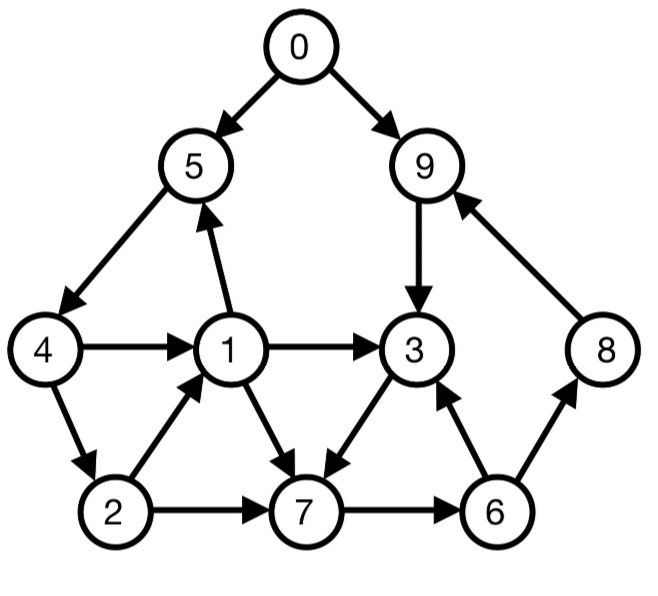
\includegraphics[width=0.65\textwidth]{graph}
        \end{center}
    \end{figure}

    \subsection{a)}
    \begin{ans}
        DFS

        \[ 0,5,4,1,3,7,6,8,9,2 \]
    \end{ans}

    \subsection{b)}
    \begin{ans} 
        Rekkefølgen på nodene når DFS er ferdig med å behandle nodene.

        \[ 9,8,6,7,3,1,2,4,5,0 \]
    \end{ans}

    \subsection{c)}

    \begin{ans}
        Gi rekkefølgen på de sterkt sammenhengende komponentene som de oppdages med Kosaraju-Sharir algoritmen.

        \[ (9,3,7,6,8) (1,5,4,2) (0) \]


    \end{ans}

    \subsection{d)}


    \begin{ans}
    Gi rekkefølgen på nodene etter første besøk iht. BFS

    \[ 0,5,9,4,3,1,2,7,6,8\]
        
    \end{ans}

    \section{Oppgave 3}

    \subsection{a)}
    Hva er kjøretiden til quicksort dersom vi alltid velger det første elementet som pivot og input er sortert i stigende rekkefølge ved start?
    \begin{ans}
        \[ O(n^2) \]
    \end{ans}

    \subsection{b)}
    Hva er kjøretiden til innsettingssortering dersom input er sortert i synkende rekkefølge ved start?

    \begin{ans}
        \[ O(n^2) \]
    \end{ans}

    \subsection{c)}

    Hva er kjøretiden til mergesort dersom input er sortert i stigende rekkefølge ved start?

    \begin{ans}
    \[ O(n \log n) \]
    \end{ans}

    \subsection{d)}
    Hva er kjøretiden til mergesort dersom input er sortert i stigende rekkefølge ved start og vi hopper over alle "merge" operasjoner av to lister A og B hvis siste elementet i A er mindre eller lik første elementet i B?
    \begin{ans}
    \[ O(n) \]
    \end{ans}


\end{document}
